\chapter{Attention Is All You Need}
\label{ch:attention}

\section{Why Attention Replaces Recurrence}

Consider the sentence: ``The cat sat on the mat because it was tired.'' The pronoun ``it'' refers to ``cat,'' seven tokens back. In an RNN, this information must survive seven sequential state updates---each one a lossy compression step. What if, instead of relaying information through a chain, each token could simply look back and ask: \emph{which earlier token am I related to?}

That question is the core of attention. Bahdanau and Luong added it on top of RNNs (Chapter~\ref{ch:before-transformer}), but the architecture still processed tokens one by one. Vaswani et al.~\cite{vaswani2017attention} asked the radical follow-up: what if attention is not an add-on, but the \emph{entire} computation? Their answer was the Transformer---a model with no recurrence at all. In unconstrained self-attention, every token attends to every other token in parallel, with $O(1)$ path length between any two positions (compared to $O(T)$ in an RNN).

This chapter builds the Transformer mechanism by mechanism, and each section answers the question left open by the previous one. We start with attention itself---and discover that it needs masking, multiple heads, positional information, and a feed-forward network before it becomes a complete architecture.

\subsection*{Learning Objectives}

After completing this chapter, you should be able to:

\begin{enumerate}
    \item Compute scaled dot-product attention by hand for a 3-token example (Q/K/V $\to$ scores $\to$ softmax $\to$ output).
    \item Explain mathematically why $\sqrt{d_k}$ scaling is necessary (dot-product variance grows with dimension).
    \item Describe how multi-head attention enables a single layer to capture multiple types of relationships simultaneously.
    \item Explain why positional encoding is necessary (attention is permutation-equivariant) and how sinusoidal encoding works.
    \item Trace the information flow through a modern pre-norm Transformer block: LayerNorm $\to$ self-attention $\to$ residual add $\to$ LayerNorm $\to$ FFN $\to$ residual add.
\end{enumerate}

\subsection*{Notation}

The following notation is introduced in this chapter and used throughout the rest of the book:

\begin{center}
\begin{tabular}{ll}
\toprule
Symbol & Meaning \\
\midrule
$\mathbf{Q}, \mathbf{K}, \mathbf{V}$ & Query, key, and value matrices \\
$d_{\text{model}}$ & Model (embedding) dimension \\
$d_k$ & Key/query dimension per head \\
$d_v$ & Value dimension per head \\
$h$ & Number of attention heads \\
$\mathbf{W}^Q, \mathbf{W}^K, \mathbf{W}^V$ & Learned projection matrices for Q, K, V \\
$\mathbf{W}^O$ & Output projection after concatenating heads \\
$\mathbf{M}$ & Attention mask matrix \\
PE$(t, i)$ & Positional encoding at position $t$, dimension $i$ \\
\bottomrule
\end{tabular}
\end{center}


\section{Scaled Dot-Product Attention}

\subsection{Query, Key, Value: Retrieval as Computation}

Consider two sentences:

\begin{quote}
\emph{The animal didn't cross the street because \textbf{it} was too wide.}\\
\emph{The animal didn't cross the street because \textbf{it} was too tired.}
\end{quote}

In both sentences, ``it'' needs to resolve what it refers to. In the first, ``wide'' makes ``street'' the correct referent; in the second, ``tired'' makes it ``animal.'' To get this right, the model processing ``it'' must \emph{look back} through the sequence and find the relevant noun---and which noun is relevant depends on context that comes later (``wide'' or ``tired'').

This is the core computational problem attention solves: \textbf{a token needs to query other tokens for information, and which tokens are relevant depends on learned, context-dependent matching.} This requires three distinct functions:

\begin{enumerate}[nosep]
    \item \textbf{Asking:} ``it'' must formulate what it is looking for (a noun that could be wide or tired).
    \item \textbf{Advertising:} ``animal'' and ``street'' must each present an identity that can be matched against.
    \item \textbf{Providing:} whichever token is selected must contribute its actual semantic content.
\end{enumerate}

These three functions correspond to three learned roles that the Transformer assigns to each token:

\begin{itemize}
    \item The \textbf{query} $\mathbf{q}$: ``what am I looking for?'' (the search request)
    \item The \textbf{key} $\mathbf{k}$: ``how should I be found?'' (the index entry)
    \item The \textbf{value} $\mathbf{v}$: ``what do I contribute if selected?'' (the retrieved content)
\end{itemize}

(Note: the coreference example above uses bidirectional context for clarity. In a causal language model, ``it'' can only attend to tokens before it. We will introduce causal masking in Section~\ref{sec:masking}; for now, focus on the retrieval mechanism itself.)

Attention then works as a differentiable lookup: it computes a similarity score between each query and all keys, normalizes these scores into weights, and returns a weighted combination of the corresponding values.

In Bahdanau attention (Chapter~\ref{ch:before-transformer}), keys and values were the same vectors---encoder hidden states served double duty as both ``what can be found'' and ``what gets returned.'' The Transformer generalizes this by using \emph{learned linear projections} to create \emph{separate} Q, K, and V representations:

\[
\mathbf{Q} = \mathbf{X}\mathbf{W}^Q, \qquad
\mathbf{K} = \mathbf{X}\mathbf{W}^K, \qquad
\mathbf{V} = \mathbf{X}\mathbf{W}^V,
\]

where $\mathbf{X} \in \mathbb{R}^{T \times d_{\text{model}}}$ is the input matrix (one row per token) and $\mathbf{W}^Q, \mathbf{W}^K \in \mathbb{R}^{d_{\text{model}} \times d_k}$, $\mathbf{W}^V \in \mathbb{R}^{d_{\text{model}} \times d_v}$ are learned projection matrices.

\paragraph{Why not use one vector for all three?} If key and value are the same vector (as in Bahdanau attention), then a token's ``findability'' is permanently tied to its ``content.'' A token that is easy to find must also provide exactly the representation it advertises. With separate projections, the model can decouple these roles: a key says ``I am a verb in past tense'' (making the token findable by queries looking for verbs), while the corresponding value provides the actual semantic content needed downstream. This decoupling is what allows attention to be a flexible, learned routing mechanism rather than a fixed similarity lookup.

\subsection{The Attention Formula}

Given $\mathbf{Q} \in \mathbb{R}^{T \times d_k}$, $\mathbf{K} \in \mathbb{R}^{T \times d_k}$, and $\mathbf{V} \in \mathbb{R}^{T \times d_v}$, scaled dot-product attention computes:

\[
\text{Attention}(\mathbf{Q}, \mathbf{K}, \mathbf{V}) = \text{softmax}\!\left(\frac{\mathbf{Q}\mathbf{K}^\top}{\sqrt{d_k}}\right) \mathbf{V}.
\]

Breaking this apart:

\begin{enumerate}
    \item $\mathbf{Q}\mathbf{K}^\top \in \mathbb{R}^{T \times T}$ computes the raw similarity between every pair of query and key vectors. Entry $(i, j)$ is the dot product $\mathbf{q}_i^\top \mathbf{k}_j$.
    \item Division by $\sqrt{d_k}$ scales the scores to control the variance.
    \item Softmax normalizes each row into a probability distribution---position $i$'s attention weights over all positions.
    \item Multiplication by $\mathbf{V}$ produces the output: a weighted average of value vectors, where the weights are the attention probabilities.
\end{enumerate}

\subsection[Why Scale by sqrt(d\_k)?]{Why Scale by $\sqrt{d_k}$?}

This is not an arbitrary constant. If the entries of $\mathbf{q}$ and $\mathbf{k}$ are independent with mean 0 and variance 1, their dot product has mean 0 and variance $d_k$:

\[
\text{Var}\!\left(\sum_{i=1}^{d_k} q_i k_i\right) = \sum_{i=1}^{d_k} \text{Var}(q_i k_i) = d_k.
\]

So the standard deviation of the dot product grows as $\sqrt{d_k}$. When $d_k$ is large (e.g., 64 or 128), the raw dot products can have large magnitude, pushing softmax into regions where its gradients are nearly zero. Dividing by $\sqrt{d_k}$ brings the variance back to approximately 1, keeping softmax in a regime where it produces informative (non-peaked) distributions and has healthy gradients.

\paragraph{A concrete example.}  Suppose $d_k = 64$ and three tokens produce raw dot-product scores $[16,\; 8,\; 7]$---plausible magnitudes when 64-dimensional vectors are involved.

\medskip
\begin{center}
\begin{tabular}{lll}
\toprule
& \textbf{Scores} & \textbf{Softmax output} \\
\midrule
Without scaling & $[16.0,\; 8.0,\; 7.0]$ & $[0.9995,\; 0.0003,\; 0.0001]$ \\
With $\sqrt{d_k} = 8$ & $[2.0,\; 1.0,\; 0.88]$ & $[0.59,\; 0.22,\; 0.19]$ \\
\bottomrule
\end{tabular}
\end{center}
\medskip

Without scaling, the model commits almost all of its attention to one token after just three scores. The other two tokens are effectively ignored. With scaling, the distribution is smoother---the model can blend information from all three sources. More importantly, softmax gradients are healthier: in the peaked regime, very small-probability entries receive tiny gradients, so backpropagation has little signal for learning that those tokens should have received more attention.

Now imagine $d_k = 512$ instead of 64. The raw scores would be even larger, and without scaling, softmax would collapse to a hard one-hot vector---effectively making attention a non-differentiable argmax. The $\sqrt{d_k}$ divisor is what keeps attention ``soft'' and trainable.

\medskip
\noindent\fbox{\parbox{\dimexpr\textwidth-2\fboxsep-2\fboxrule\relax}{\textbf{Intuition checkpoint.} In the unscaled row above, the second-best token gets only about 0.03\% of the weight. What happens to the gradient of that token's score? If the gradient is tiny, can the model easily learn to shift attention toward it in future training steps?}}
\medskip

\subsection{A Toy Example: Hand-Computing Attention}

We will use the same 3-token example throughout this chapter: ``the cat sat,'' with $d_{\text{model}} = 4$ and $d_k = d_v = 2$. Suppose after projection:

\[
\mathbf{Q} = \begin{pmatrix} 1 & 0 \\ 0 & 1 \\ 1 & 1 \end{pmatrix}, \quad
\mathbf{K} = \begin{pmatrix} 1 & 1 \\ 0 & 1 \\ 1 & 0 \end{pmatrix}, \quad
\mathbf{V} = \begin{pmatrix} 1 & 0 \\ 0 & 1 \\ 1 & 1 \end{pmatrix}.
\]

\paragraph{Step 1: Compute $\mathbf{Q}\mathbf{K}^\top$.}

\[
\mathbf{Q}\mathbf{K}^\top = \begin{pmatrix} 1 & 0 & 1 \\ 1 & 1 & 0 \\ 2 & 1 & 1 \end{pmatrix}.
\]

\paragraph{Step 2: Scale by $\sqrt{d_k} = \sqrt{2} \approx 1.41$.}

\[
\frac{\mathbf{Q}\mathbf{K}^\top}{\sqrt{2}} \approx \begin{pmatrix} 0.71 & 0 & 0.71 \\ 0.71 & 0.71 & 0 \\ 1.41 & 0.71 & 0.71 \end{pmatrix}.
\]

\paragraph{Step 3: Softmax (row-wise).}\mbox{}

\medskip
\noindent\fbox{\parbox{\dimexpr\textwidth-2\fboxsep-2\fboxrule\relax}{\textbf{Pause and predict.} Before looking at the softmax output, examine the scaled score matrix above. Row~3 (``sat'') has scores 1.41, 0.71, 0.71. Which token will ``sat'' attend to most strongly? By how much? Make your prediction, then continue.}}
\medskip

\[
\text{softmax} \approx \begin{pmatrix} 0.39 & 0.19 & 0.39 \\ 0.39 & 0.39 & 0.19 \\ 0.50 & 0.25 & 0.25 \end{pmatrix}.
\]

\paragraph{How to read the attention matrix.} Before computing the final output, pause and read the softmax matrix---it reveals how the model ``thinks'':

\begin{itemize}[nosep]
    \item Each \textbf{row} is a query token asking ``who should I attend to?''
    \item Each \textbf{column} is a key token being asked ``how relevant are you?''
    \item The \textbf{weights} are determined entirely by Q$\cdot$K dot products---V plays no role in deciding \emph{who} gets attended to.
\end{itemize}

Look at row 3 (``sat''): it assigns weight 0.50 to ``the'' and only 0.25 each to ``cat'' and ``sat.'' Why? Because sat's query vector $(1,1)$ has the highest dot product with the's key vector $(1,1)$---a score of 2, versus 1 for the other keys. \textbf{The query-key match decides the routing; the value decides the content.} This is the fundamental separation that makes attention powerful: what a token ``looks for'' (query) and what it ``provides when found'' (value) are independent.

\paragraph{Step 4: Multiply by $\mathbf{V}$.}

The output for ``the'' (row 1) is $0.39 \cdot (1,0) + 0.19 \cdot (0,1) + 0.39 \cdot (1,1) = (0.78, 0.58)$: a blend of all three value vectors, weighted by the attention scores. Notice that every output position has been informed by every input position---in a single step, with no serial dependency.

\begin{figure}[ht]
\centering
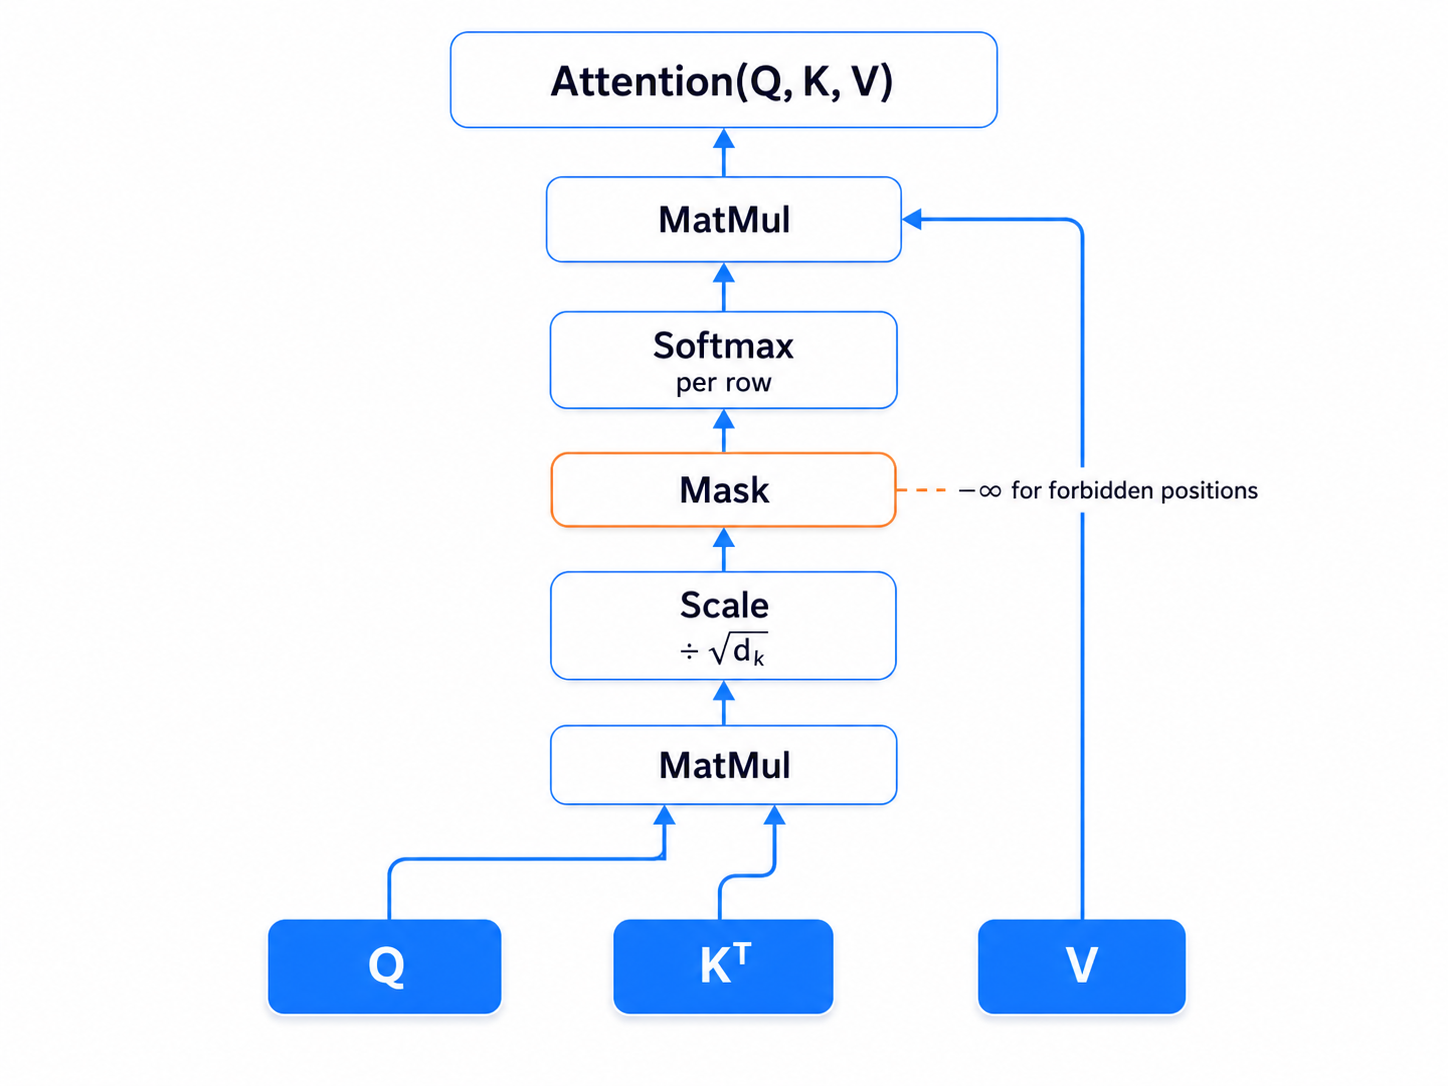
\includegraphics[width=0.85\textwidth]{figures/ch02/scaled_dot_product_attention.png}
\caption{Scaled dot-product attention. Queries and keys are multiplied to produce a score matrix, which is scaled by $\sqrt{d_k}$, optionally masked (Section~\ref{sec:masking}), and normalized by softmax. The resulting attention weights select a weighted combination of value vectors. The orange-highlighted mask step is where causal constraints are enforced.}
\label{fig:scaled-dot-product}
\end{figure}

\begin{quickrecap}
\textbf{Quick Recap.}
\begin{itemize}[nosep,leftmargin=1.5em]
  \item Attention is three-step retrieval: Q$\cdot$K similarity $\to$ softmax $\to$ weighted average of V.
  \item $\sqrt{d_k}$ scaling prevents dot products from growing with dimension, avoiding softmax saturation.
  \item Every output position is informed by every input position in one parallel step---no serial dependency.
  \item \textbf{But:} ``every position sees every position'' is a problem for language modeling---token $t$ should not see token $t{+}1$ when predicting it.
\end{itemize}
\end{quickrecap}


\section{Masking: What Tokens Can See}
\label{sec:masking}

In an RNN, causality is \emph{built into the computation order}: $\mathbf{h}_t$ depends only on $\mathbf{h}_{t-1}$ and $\mathbf{x}_t$, so token $t$ cannot possibly access token $t{+}1$. There is no way to break this even if you tried. In a Transformer, there is no such structural guarantee---self-attention connects \emph{every} position to \emph{every} other position by default. Causality must be \emph{externally imposed} through a mask. This is precisely why mask bugs are a Transformer-specific problem: the architecture's default is bidirectional, and any mistake in the mask silently leaks future information.

\subsection{Causal (Autoregressive) Mask}

In a language model, token $t$ must predict token $t+1$ using only positions $1, \ldots, t$. It must \emph{not} see positions $t+1, \ldots, T$---that would be cheating. The causal mask enforces this by setting the upper triangle of the score matrix to $-\infty$ before softmax:

\[
\mathbf{M}_{ij} = \begin{cases} 0 & \text{if } j \leq i \\ -\infty & \text{if } j > i \end{cases}
\]

After adding $\mathbf{M}$ to the raw scores:

\[
\text{Attention}(\mathbf{Q}, \mathbf{K}, \mathbf{V}) = \text{softmax}\!\left(\frac{\mathbf{Q}\mathbf{K}^\top}{\sqrt{d_k}} + \mathbf{M}\right) \mathbf{V}.
\]

The $-\infty$ entries become 0 after softmax, so the model cannot attend to future tokens. Continuing our toy example:

\[
\frac{\mathbf{Q}\mathbf{K}^\top}{\sqrt{2}} + \mathbf{M} \approx \begin{pmatrix} 0.71 & -\infty & -\infty \\ 0.71 & 0.71 & -\infty \\ 1.41 & 0.71 & 0.71 \end{pmatrix}.
\]

After softmax: row 1 assigns all weight to position 1; row 2 splits between positions 1 and 2; row 3 distributes across all three positions. ``The'' can only see itself; ``cat'' can see ``the'' and ``cat''; ``sat'' can see everything.

\begin{figure}[ht]
\centering
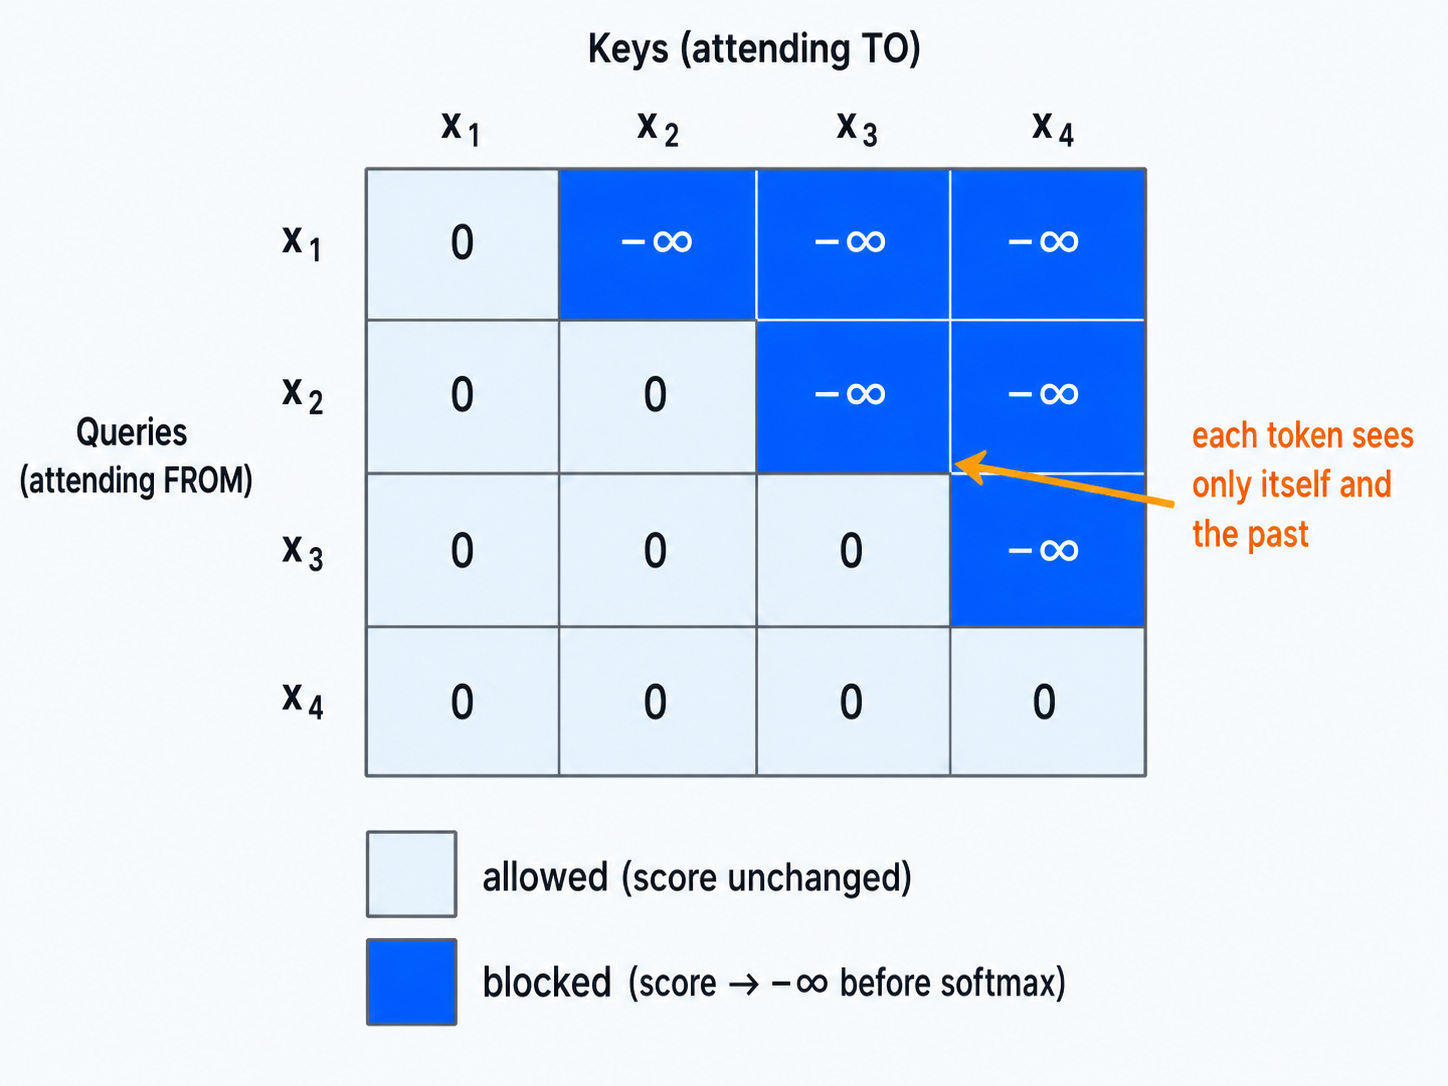
\includegraphics[width=0.75\textwidth]{figures/ch02/causal_mask.png}
\caption{Causal (autoregressive) mask for a 4-token sequence. White cells (score unchanged) allow attention; blue cells (score set to $-\infty$) block it. Each token can attend only to itself and earlier positions, preventing future information from leaking into predictions.}
\label{fig:causal-mask}
\end{figure}

\subsection{Padding Mask}

When batching sequences of different lengths, shorter sequences are padded to the batch maximum. Padding tokens carry no information, so they must be excluded from attention. A padding mask sets attention scores to $-\infty$ for all positions that correspond to padding tokens.

\subsection{Implementation Pitfalls}

Masking is the most common source of silent bugs in Transformer implementations:

\begin{itemize}
    \item \textbf{Mask polarity.} Some frameworks use \texttt{True} for ``attend,'' others for ``mask out.'' In PyTorch's \texttt{nn.MultiheadAttention}, a \texttt{True} value in the mask means ``do \emph{not} attend.'' Getting this backwards means future tokens leak into predictions.
    \item \textbf{Where to apply.} The mask must be added to the raw scores \emph{before} softmax, not after. Zeroing attention weights post-softmax does not work: the remaining weights no longer sum to 1, and the masked positions still influenced the softmax normalization.
    \item \textbf{Combined masks.} In practice, causal and padding masks are combined (additive or logical \texttt{OR}). Forgetting either one is a bug. A missing causal mask causes future-token leakage; a missing padding mask causes padding to pollute real tokens.
    \item \textbf{The symptom.} Suppose you train a 6-layer Transformer LM on WikiText-103 and get validation perplexity of 1.8. Published results for similar-sized models report PPL in the tens, not near 1. Your model appears an order of magnitude better than the state of the art---something is wrong. The cause: a missing causal mask lets the model ``predict'' tokens it has already seen. During inference, when the mask is correctly applied (because future tokens do not exist yet), the model performs terribly---it never learned to work without future information.
\end{itemize}

\medskip
\noindent\fbox{\parbox{\dimexpr\textwidth-2\fboxsep-2\fboxrule\relax}{\textbf{Intuition checkpoint.} You train a language model and notice that validation perplexity is 1.5---far lower than any published result for your model size. What is the most likely cause? How would you verify your hypothesis?}}
\medskip

\begin{quickrecap}
\textbf{Quick Recap.}
\begin{itemize}[nosep,leftmargin=1.5em]
  \item Causal mask (lower-triangular) prevents future-token leakage; padding mask excludes filler tokens.
  \item Masks must be applied \emph{before} softmax as $-\infty$ additive terms, not after.
  \item Missing causal mask = most common silent bug: training loss looks good, but model cannot generate.
  \item \textbf{But:} even with correct masking, a single attention head can only capture one type of relationship at a time.
\end{itemize}
\end{quickrecap}


\section{Multi-Head Attention}

\subsection{Motivation: One Head Is Not Enough}

A single attention head computes one set of attention weights, meaning each position forms one ``query'' and identifies one pattern of relevant positions. But language involves multiple simultaneous relationships: syntactic (subject-verb), semantic (entity-attribute), positional (local adjacency). A single head must compromise across all of these.

\subsection{Mechanism}

Multi-head attention runs $h$ independent attention functions in parallel, each with its own learned projections:

\[
\text{head}_i = \text{Attention}(\mathbf{X}\mathbf{W}_i^Q, \, \mathbf{X}\mathbf{W}_i^K, \, \mathbf{X}\mathbf{W}_i^V),
\]

where $\mathbf{W}_i^Q, \mathbf{W}_i^K \in \mathbb{R}^{d_{\text{model}} \times d_k}$ and $\mathbf{W}_i^V \in \mathbb{R}^{d_{\text{model}} \times d_v}$, with $d_k = d_v = d_{\text{model}} / h$.

The outputs of all heads are concatenated and projected:

\[
\text{MultiHead}(\mathbf{X}) = \text{Concat}(\text{head}_1, \ldots, \text{head}_h)\, \mathbf{W}^O,
\]

where $\mathbf{W}^O \in \mathbb{R}^{hd_v \times d_{\text{model}}}$.

\subsection{Parameter Count}

A key design choice: $d_k = d_{\text{model}} / h$. This means that multi-head attention with $h$ heads has approximately the same total parameter count as single-head attention with full $d_{\text{model}}$ dimensions:

\[
\underbrace{h \cdot 3 \cdot d_{\text{model}} \cdot \frac{d_{\text{model}}}{h}}_{\text{Q, K, V projections}} + \underbrace{d_{\text{model}}^2}_{\mathbf{W}^O} = 4 \, d_{\text{model}}^2.
\]

You get $h$ different ``views'' of the data for approximately the same computational budget as one view. This is not free---each head has lower-dimensional projections, so individual heads have less capacity---but empirically the diversity of multiple heads more than compensates.

\begin{figure}[ht]
\centering
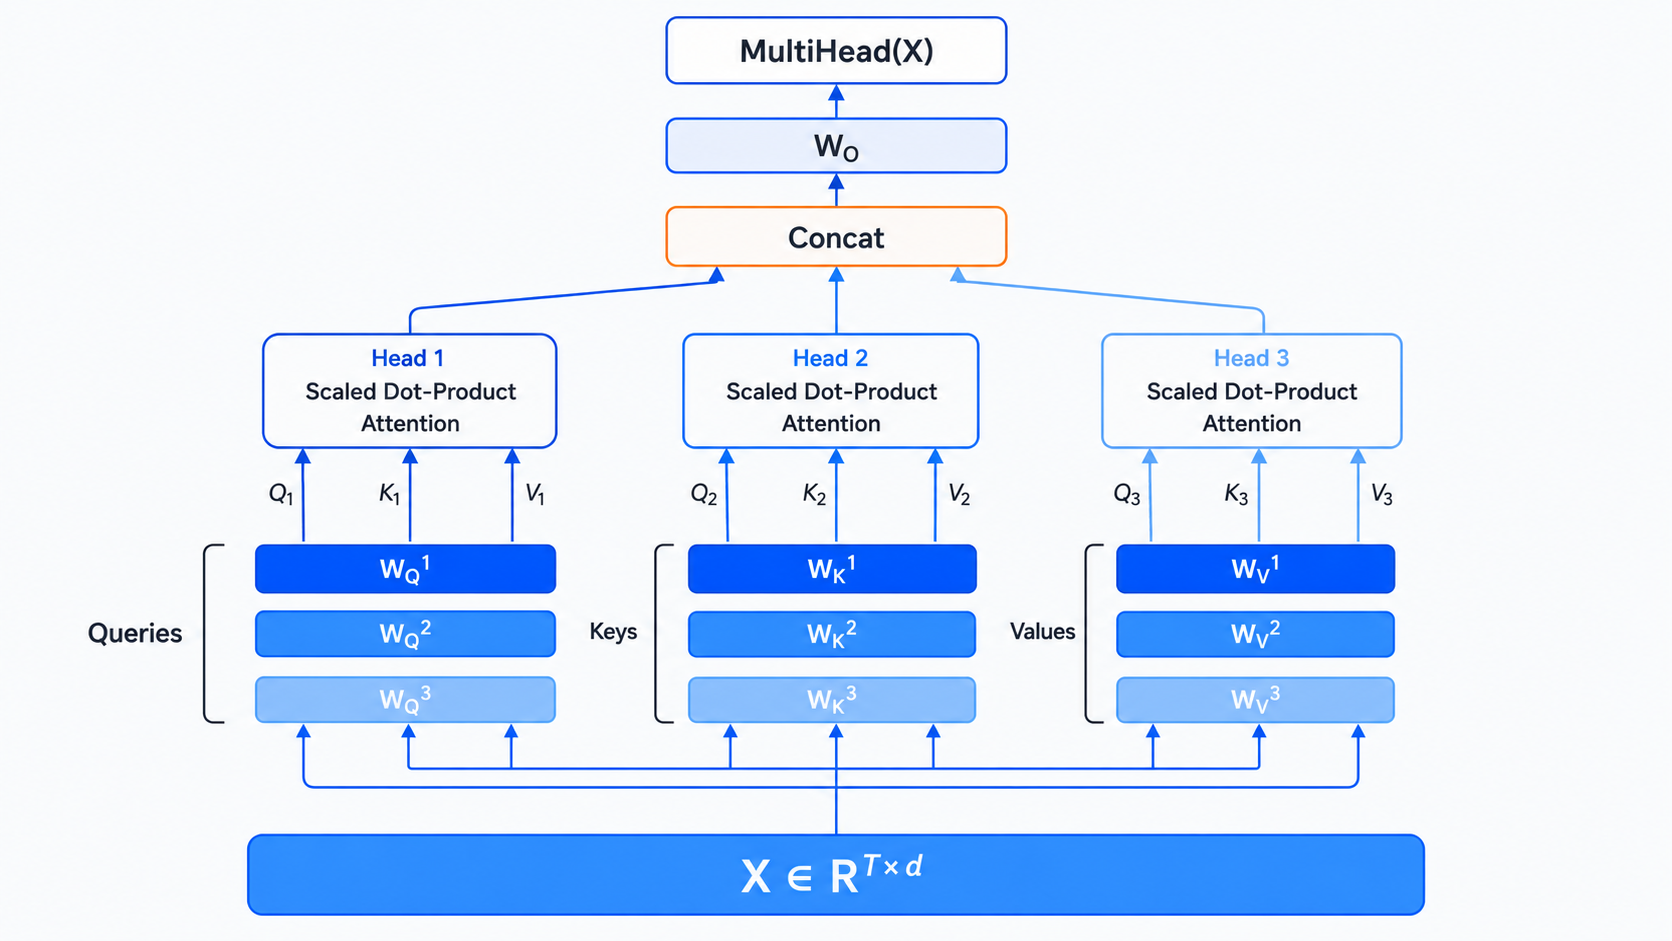
\includegraphics[width=0.85\textwidth]{figures/ch02/multi_head_attention.png}
\caption{Multi-head attention with $h = 3$ heads. The input $\mathbf{X}$ is projected into separate Q, K, V spaces by each head's learned weight matrices. Each head independently computes scaled dot-product attention, and the outputs are concatenated and projected through $\mathbf{W}^O$ to produce the final result. Different heads can specialize in different relationship types (syntactic, semantic, positional).}
\label{fig:multi-head}
\end{figure}

\medskip
\noindent\fbox{\parbox{\dimexpr\textwidth-2\fboxsep-2\fboxrule\relax}{\textbf{Intuition checkpoint.} If you set $h = d_{\text{model}}$ (one head per dimension), each head would use scalar dot products. Would this work? What would be lost compared to, say, $h = 8$ with $d_k = d_{\text{model}} / 8$?}}
\medskip

\begin{quickrecap}
\textbf{Quick Recap.}
\begin{itemize}[nosep,leftmargin=1.5em]
  \item Multi-head: $h$ independent attention functions in parallel, each with its own Q/K/V projections.
  \item With $d_k = d_{\text{model}}/h$, total parameters $\approx$ same as single-head.
  \item Different heads capture different relationships (syntactic, semantic, positional).
  \item \textbf{But:} attention treats the input as a \emph{set}, not a sequence---it has no concept of word order.
\end{itemize}
\end{quickrecap}


\section{Positional Information}

\subsection{The Problem: Attention Is Position-Blind}

Self-attention is \emph{permutation-equivariant}: if you shuffle the rows of the input matrix $\mathbf{X}$, the output rows shuffle in exactly the same way. This means that, without additional information, the model cannot distinguish ``the cat sat'' from ``sat the cat'' or ``cat sat the.'' For language, word order is essential.

To see this formally: the attention computation $\text{softmax}(\mathbf{Q}\mathbf{K}^\top / \sqrt{d_k})\mathbf{V}$ depends only on the pairwise dot products of projected rows. If rows are permuted, the dot products (and therefore the attention weights) are permuted identically. The output at position $i$ has no way to ``know'' that it is position $i$ rather than position $j$.

\subsection{Sinusoidal Positional Encoding}

Vaswani et al.\ inject positional information by adding a fixed positional encoding to the input embeddings:

\[
\text{PE}(t, 2i) = \sin\!\left(\frac{t}{10000^{2i/d_{\text{model}}}}\right), \qquad
\text{PE}(t, 2i+1) = \cos\!\left(\frac{t}{10000^{2i/d_{\text{model}}}}\right).
\]

Why sinusoidal functions specifically? Because their product-to-sum identities mean that the dot product between PE vectors at positions $t$ and $t{+}k$ depends only on the offset $k$, not on $t$ itself. This lets the model learn relative-position patterns (``the word 3 positions back'') from absolute positional encodings.

Each dimension $i$ oscillates at a different frequency. Think of a row of clocks: the second hand spins fast (low dimensions), the minute hand spins slower (middle dimensions), and the hour hand barely moves (high dimensions). By reading all the hands together, you can uniquely identify any time---and by reading all PE dimensions, the model can uniquely identify any position. The key properties are:

\begin{itemize}
    \item Every position gets a unique encoding.
    \item The encoding for position $t + k$ can be expressed as a linear function of the encoding at position $t$, which makes it possible for attention to learn relative-position patterns.
    \item The encoding generalizes to sequence lengths not seen during training (unlike learned embeddings, which are fixed to the training length).
\end{itemize}

\subsection{Learned Positional Embeddings}

An alternative is to learn a position embedding matrix $\mathbf{P} \in \mathbb{R}^{T_{\max} \times d_{\text{model}}}$ alongside the token embeddings. This is simpler and performs comparably for fixed-length settings. The disadvantage is that the model cannot generalize beyond $T_{\max}$ positions.

\subsection{Beyond Fixed Encodings}

Modern Transformer variants have introduced more sophisticated positional methods. Rotary Position Embedding (RoPE) encodes relative position directly into the attention computation by rotating query and key vectors; ALiBi adds a learned bias proportional to distance. We cover these in detail in later chapters when we discuss long-context modeling. For now, the important point is: \emph{some} mechanism for injecting position is necessary, and the choice affects both context length and quality.

\subsection{An Asymmetry: Causal Mask as Implicit Position}
\label{sec:causal-mask-implicit-position}

The opening of this section claimed that self-attention is permutation-equivariant, so position information must be explicitly injected. That statement is true \emph{only for bidirectional (encoder) self-attention}. \emph{Causal} self-attention (decoder side) is a different story: by construction, position $t$ can attend to positions $1, 2, \ldots, t$ but not to $t+1, \ldots, T$. The number of attendable predecessors is itself a positional signal, and the attention pattern between mask-induced subsets is no longer permutation-equivariant. The model can learn to read absolute position off the mask alone.

\medskip
\noindent\fbox{\parbox{\dimexpr\textwidth-2\fboxsep-2\fboxrule\relax}{\textbf{Empirical anchor.} Haviv et al.~\cite{haviv2022nope} showed that a decoder-only language model trained \emph{without any explicit positional encoding} is essentially competitive with a standard PE-equipped model. Probing experiments confirm the model encodes absolute position throughout its layers. Lab~2 Experiment~3 reproduces this asymmetry on a different task: removing encoder PE drops accuracy from 97\% to 22\%, while removing decoder PE drops it by less than one point.}}
\medskip

The intuition is simple: every decoder position sees a strictly different number of context tokens, so different positions have measurably different attention statistics. The encoder, in contrast, has no such structural difference --- every position sees every other --- and is genuinely permutation-equivariant without explicit positional input.

This asymmetry matters in practice. For an encoder-only model (BERT-style), explicit positional encoding is non-negotiable. For a decoder-only model (GPT-style), the choice of positional encoding is a tunable design decision, and the ``no positional encoding'' (NoPE) baseline is a real option worth considering, especially for length-generalization-sensitive applications~\cite{kazemnejad2023impact}. We return to this in Chapter~\ref{ch:decoder-only}.

\begin{quickrecap}
\textbf{Quick Recap.}
\begin{itemize}[nosep,leftmargin=1.5em]
  \item Self-attention is permutation-equivariant: without positional info, it cannot distinguish word order.
  \item Sinusoidal encoding: fixed sine/cosine waves; learned embeddings: simpler but cannot extrapolate.
  \item Modern methods (RoPE) encode \emph{relative} position directly in the attention computation.
  \item \textbf{Asymmetry:} the permutation-equivariance argument applies only to bidirectional attention. Causal (decoder) self-attention encodes position implicitly via the mask; explicit PE on the decoder side is partially redundant.
  \item \textbf{But:} for fixed attention weights, attention outputs a weighted average of V. Where does nonlinearity come from?
\end{itemize}
\end{quickrecap}


\section{The Transformer Block}

\subsection{Architecture}

A Transformer block consists of two sub-layers, each wrapped in a residual connection and layer normalization:

\begin{enumerate}
    \item \textbf{Multi-head self-attention} (MHA): each position attends to all (visible) positions.
    \item \textbf{Position-wise feed-forward network} (FFN): a two-layer MLP applied independently to each position.
\end{enumerate}

In the original (post-norm) formulation:

\begin{align}
\mathbf{Z} &= \text{LayerNorm}\!\big(\mathbf{X} + \text{MHA}(\mathbf{X})\big), \\
\mathbf{Y} &= \text{LayerNorm}\!\big(\mathbf{Z} + \text{FFN}(\mathbf{Z})\big),
\end{align}

where the FFN is:

\[
\text{FFN}(\mathbf{z}) = \mathbf{W}_2\, \text{ReLU}(\mathbf{W}_1 \mathbf{z} + \mathbf{b}_1) + \mathbf{b}_2.
\]

The inner dimension of the FFN is typically $4 \times d_{\text{model}}$, so $\mathbf{W}_1 \in \mathbb{R}^{d_{\text{model}} \times 4d_{\text{model}}}$ and $\mathbf{W}_2 \in \mathbb{R}^{4d_{\text{model}} \times d_{\text{model}}}$.

\subsection{Residual Connections}

The residual connection $\mathbf{X} + \text{MHA}(\mathbf{X})$ serves the same purpose as the LSTM cell state highway from Chapter~\ref{ch:before-transformer}: it provides a near-identity path through the network, allowing gradients to flow backward through many layers without vanishing. Without residual connections, training deep Transformers (12+ layers) becomes extremely difficult.

\subsection{Layer Normalization}

Layer normalization stabilizes training by normalizing each token's representation across its feature dimensions to zero mean and unit variance. The original Transformer used \emph{post-norm} (normalize after the residual addition), but most modern implementations use \emph{pre-norm} (normalize before the sub-layer):

\begin{align}
\mathbf{Z} &= \mathbf{X} + \text{MHA}\!\big(\text{LayerNorm}(\mathbf{X})\big), \\
\mathbf{Y} &= \mathbf{Z} + \text{FFN}\!\big(\text{LayerNorm}(\mathbf{Z})\big).
\end{align}

Pre-norm is easier to train at depth because the residual path is cleaner (no normalization between the skip and the output). We discuss the training stability implications in Chapter~4.

\begin{figure}[ht]
\centering
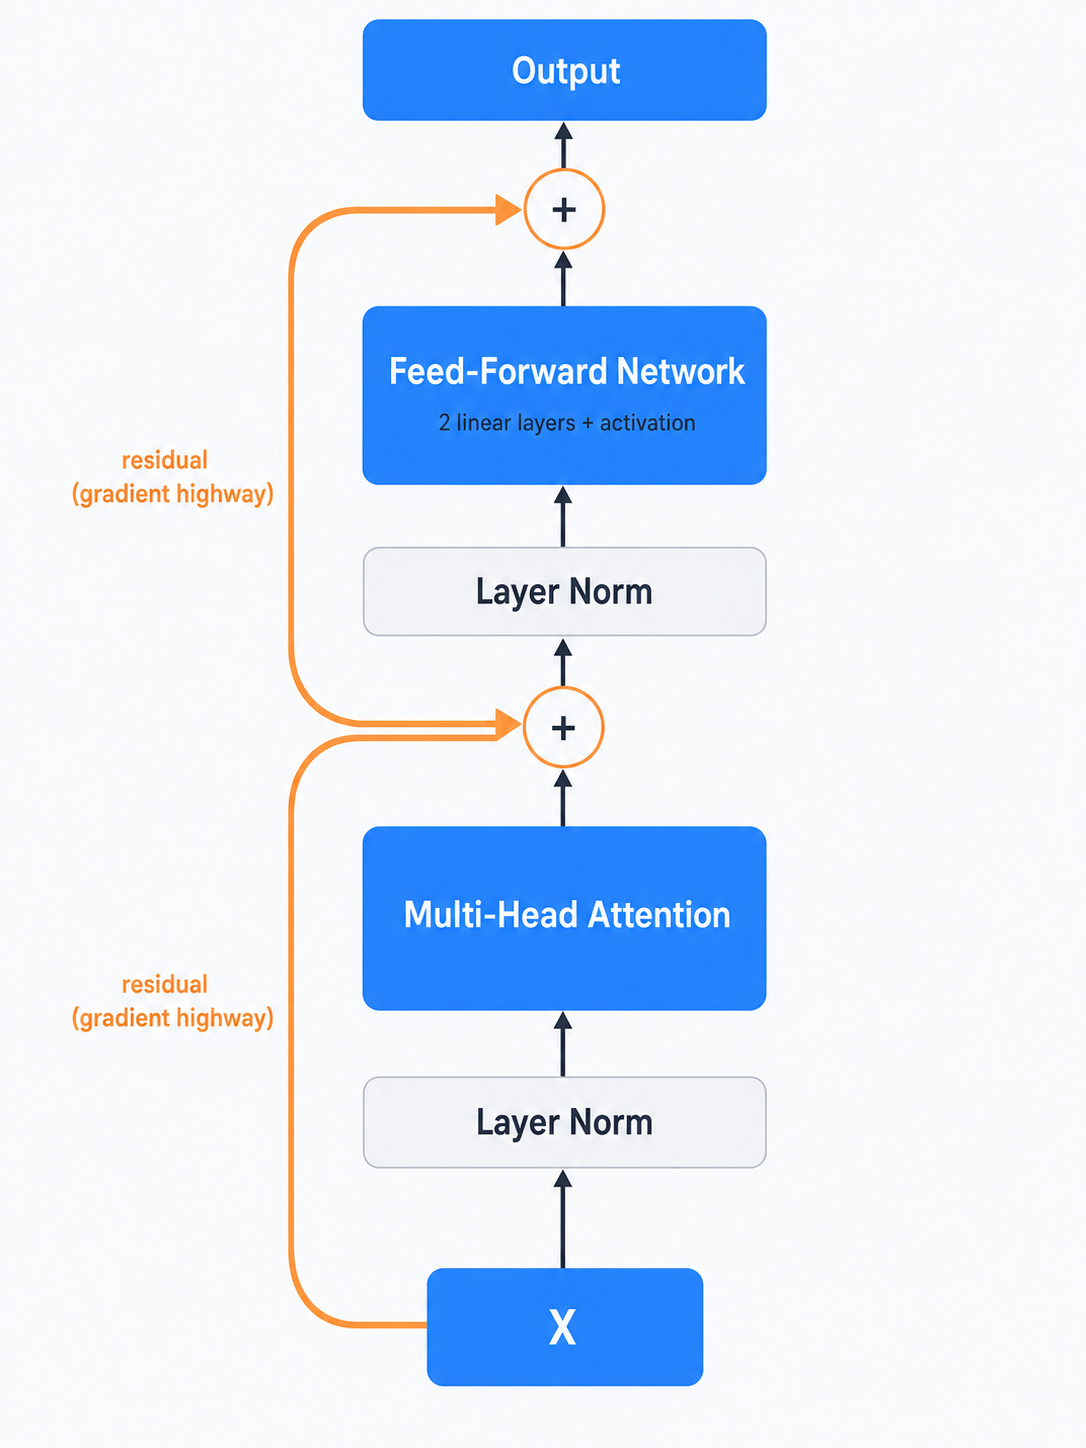
\includegraphics[width=0.55\textwidth]{figures/ch02/transformer_block.png}
\caption{A pre-norm Transformer block. The input passes through Layer Normalization before each sub-layer (MHA and FFN). The orange residual (skip) connections bypass both sub-layers, providing a gradient highway analogous to the LSTM cell state path (Chapter~\ref{ch:before-transformer}). This architecture is used in most modern LLMs.}
\label{fig:transformer-block}
\end{figure}

\subsection{The FFN's Role: Why Two-Thirds of the Parameters Are Not in Attention}

It is tempting to view the FFN as an afterthought---after all, the paper is called ``Attention Is All You Need.'' But the FFN accounts for roughly two-thirds of a Transformer's parameters, and removing it significantly degrades performance. Why?

\textbf{Attention routes; the FFN transforms.} Attention is an \emph{inter-token} operation: it decides which positions are relevant and produces a weighted average of their value vectors. But for fixed attention weights, this aggregation is a weighted linear combination of value vectors---it can blend information but cannot create new nonlinear features from it. The FFN is a \emph{per-token} (intra-token) operation: it takes the information that attention gathered and transforms it through a nonlinear function.

\textbf{Why two layers?} A single linear layer after attention could largely be folded into surrounding linear projections---it would add little expressiveness. The ReLU (or GELU/SiLU in modern variants) between $\mathbf{W}_1$ and $\mathbf{W}_2$ is what makes the FFN meaningful. The ``expand then compress'' shape ($d_\text{model} \to 4d_\text{model} \to d_\text{model}$) gives the model a higher-dimensional space in which to apply the nonlinearity before projecting back.

\textbf{An analogy.} If attention is a meeting where people share information, the FFN is the individual thinking that happens after the meeting---each person (token) privately processes what they heard and updates their understanding. Both steps are essential: without the meeting, tokens are isolated; without the private processing, they cannot integrate what they learned.

\medskip
\noindent\fbox{\parbox{\dimexpr\textwidth-2\fboxsep-2\fboxrule\relax}{\textbf{Intuition checkpoint.} A Transformer block has two residual paths. If you removed both---so the block became $\mathbf{Y} = \text{FFN}(\text{MHA}(\mathbf{X}))$ without any skip connections---what would happen when stacking 24 such blocks? (Hint: think about what happens to gradient magnitude as it passes through 24 matrix multiplications.)}}
\medskip

\begin{quickrecap}
\textbf{Quick Recap.}
\begin{itemize}[nosep,leftmargin=1.5em]
  \item Transformer block (pre-norm): LayerNorm $\to$ MHA $\to$ residual $\to$ LayerNorm $\to$ FFN $\to$ residual.
  \item Residual connections = gradient highway through depth (same role as LSTM cell state).
  \item FFN provides per-token nonlinearity that attention's weighted averaging cannot.
  \item Pre-norm is easier to train at depth than post-norm.
\end{itemize}
\end{quickrecap}


\section{What Attention Costs}

Attention enables parallel computation and direct long-range interaction. But it is not free.

\subsection{Time and Memory Complexity}

The attention score matrix $\mathbf{Q}\mathbf{K}^\top$ has shape $T \times T$. Computing and storing it costs $O(T^2 d_k)$ time and $O(T^2)$ memory. For comparison, an RNN processes a sequence in $O(T d^2)$ time and $O(d)$ memory per step.

The pairwise attention term is modest at short sequence lengths, but it dominates as $T$ grows. To feel the numbers: at $T = 4{,}096$, each attention head stores a $4{,}096 \times 4{,}096 = 16.8\text{M}$ entry score matrix. A 32-head, 32-layer model computes 1{,}024 such matrices per forward pass---over 17 billion entries just for attention scores. At $T = 100{,}000$, each matrix has 10 billion entries, and the problem becomes severe.

\subsection{The Parallelism--Cost Tradeoff}

The quadratic cost is the price of direct interaction: every token can attend to every other token. An RNN has linear complexity but serial computation. The Transformer's advantage is not that it does less work---it is that the work is \emph{parallelizable}. On modern hardware (GPUs, TPUs), parallel matrix multiplications are vastly more efficient than serial operations, so the Transformer's wall-clock time is much lower despite doing more total FLOPs for long sequences.

\subsection{Looking Ahead}

The quadratic bottleneck has motivated extensive research into efficient attention variants: sparse attention, linear attention, FlashAttention (which reduces memory but not asymptotic complexity), and KV caching for autoregressive inference. We cover KV caching and inference optimization in later chapters on serving and long-context modeling. For now, the important takeaway is:

\begin{quote}
Attention replaced the serial bottleneck of RNNs with a quadratic cost in sequence length. This tradeoff is favorable for the sequence lengths used in pretraining (2k--8k tokens) but becomes problematic at longer contexts.
\end{quote}

\begin{quickrecap}
\textbf{Quick Recap.}
\begin{itemize}[nosep,leftmargin=1.5em]
  \item Attention costs $O(T^2 d_k)$ time and $O(T^2)$ memory per layer.
  \item The pairwise $T^2$ term is modest at short lengths but dominates at long contexts.
  \item Key advantage is not lower FLOPs but \emph{parallelizability}: $T^2$ matrix ops saturate GPUs far better than serial $T$-step chains.
\end{itemize}
\end{quickrecap}

\section{Failure Modes and Common Misconceptions}

\begin{itemize}
    \item \textbf{``Attention learns word relationships.''} More precisely, attention learns \emph{projected} relationships. The raw token embeddings do not interact directly---they are first projected through learned $\mathbf{W}^Q$, $\mathbf{W}^K$, $\mathbf{W}^V$ matrices. Two tokens might be similar in embedding space but have very different query-key interactions after projection. This is a feature: it lets the model learn task-specific notions of relevance.

    \item \textbf{``More heads are always better.''} Increasing $h$ while keeping $d_{\text{model}}$ fixed reduces $d_k = d_{\text{model}} / h$, giving each head fewer dimensions to work with. Empirically, there is a sweet spot: too few heads limit the diversity of attention patterns, but too many heads reduce per-head capacity below a useful threshold. For GPT-scale models, $h = 32$--$96$ with $d_k = 64$--$128$ is typical.

    \item \textbf{``The Transformer has no inductive bias for sequences.''} This is half-right. The architecture itself is permutation-equivariant, but positional encoding injects sequence structure. The \emph{nature} of the inductive bias is different from RNNs: RNNs have a built-in recency bias (recent tokens have stronger influence by construction); Transformers treat all positions symmetrically and must learn any locality or recency preference from data.

    \item \textbf{``Attention is $O(T^2)$, so Transformers cannot handle long sequences.''} The quadratic cost is real, but FlashAttention and related techniques reduce the memory overhead to $O(T)$ by recomputing attention on the fly, and KV caching makes autoregressive inference $O(T)$ per step. The computational cost is still quadratic, but practical long-context Transformers (128k+ tokens) exist and are widely deployed.

    \item \textbf{``Self-attention is all you need.''} Despite the paper title, the FFN sub-layer is essential. Ablation studies show that removing the FFN significantly degrades performance. Attention selects and routes information; the FFN transforms it.
\end{itemize}


\section{Trick Table}

\noindent
\begin{tabularx}{\textwidth}{@{}>{\raggedright\arraybackslash}p{2.8cm}
                              >{\raggedright\arraybackslash}p{2.8cm}
                              >{\raggedright\arraybackslash}p{3.2cm}
                              X@{}}
\toprule
\textbf{Trick} & \textbf{When to use} & \textbf{Expected effect} & \textbf{Failure signal} \\
\midrule
$\sqrt{d_k}$ scaling &
  Always; part of the standard attention formula &
  Prevents softmax saturation; maintains gradient flow &
  Attention weights become nearly one-hot; loss plateaus \\[4pt]
Causal mask &
  Any autoregressive (decoder) model &
  Prevents future-token information leakage &
  Suspiciously low val loss; poor generation quality \\[4pt]
Pre-norm (vs.\ post-norm) &
  Deep Transformers ($\geq 12$ layers) &
  Easier optimization; avoids loss spikes early in training &
  Post-norm may diverge without careful LR warmup \\[4pt]
Attention dropout &
  Regularization during training; typical 0.1 &
  Prevents heads from co-adapting; improves generalization &
  Too high: underfitting. Too low: overfitting \\[4pt]
Head pruning / analysis &
  After training; diagnostics &
  Identifies redundant heads; enables model compression &
  Pruning load-bearing heads degrades specific capabilities \\
\bottomrule
\end{tabularx}


\begin{takeaways}
\begin{itemize}[leftmargin=1.2em, itemsep=4pt]
  \item Attention is \textbf{content-based parallel retrieval}: each query retrieves a weighted combination of values, where the weights are determined by query-key similarity.
  \item The $\sqrt{d_k}$ scaling prevents dot products from growing with dimension, which would push softmax into near-one-hot saturation and kill gradients.
  \item \textbf{Masking is where silent bugs live.} A missing causal mask lets the model see future tokens during training—loss looks good, but generation is broken. Always verify mask correctness before trusting training metrics.
  \item Multi-head attention lets different heads specialize in different relationship types (syntactic, positional, semantic) using separate learned projections of the same input.
  \item Without positional encoding, attention is \emph{permutation-equivariant}: it cannot distinguish ``the cat sat'' from ``sat cat the.'' Position information must be explicitly injected.
  \item A Transformer block = MHA + FFN + residual connections + LayerNorm. The residual paths are gradient highways (same principle as LSTM cell state); the FFN provides per-token nonlinearity that attention alone cannot.
  \item Attention costs $O(T^2)$ in sequence length—the price of letting every token see every other token. This is favorable at typical pretraining lengths but becomes the bottleneck for long contexts.
\end{itemize}
\end{takeaways}

\section{Summary}

Chapter~\ref{ch:before-transformer} diagnosed the problem: recurrent architectures compress context through a serial bottleneck that limits parallelism, effective range, and gradient flow. This chapter presented the solution: \textbf{attention as the sole mechanism for token interaction}, replacing sequential state updates with parallel, content-based retrieval.

But a mechanism is not yet a model. The original Transformer paper~\cite{vaswani2017attention} used these mechanisms in an \emph{encoder--decoder} architecture for machine translation: the encoder uses bidirectional self-attention, the decoder uses causal self-attention plus cross-attention to the encoder. GPT~\cite{radford2018improving} later showed that a \emph{decoder-only} Transformer is sufficient for powerful language modeling, while BERT~\cite{devlin2019bert} showed that an \emph{encoder-only} Transformer excels at understanding tasks. Three architectures, all built from the same attention mechanism---but with very different masking strategies and training objectives.

Several questions remain open:

\begin{itemize}[nosep]
    \item Why did decoder-only Transformers win over encoder--decoder and encoder-only alternatives for LLMs?
    \item What design choices---depth, width, activation function, normalization---define a modern GPT-style model?
    \item How do you actually \emph{train} a Transformer at scale---learning rate schedules, initialization, mixed precision?
\end{itemize}

These are the subjects of Chapters~3 and~4. The attention mechanism you learned here is the engine; the next chapters show you the car.

\medskip
\noindent\textit{Self-check: revisit the Learning Objectives. Can you compute scaled dot-product attention by hand? Can you explain $\sqrt{d_k}$ scaling, multi-head motivation, positional encoding necessity, and the role of each component in a Transformer block? If any point is unclear, re-read the corresponding section before continuing.}


\section*{Key Equations at a Glance}

\begin{center}
\renewcommand{\arraystretch}{1.6}
\begin{tabularx}{\textwidth}{@{}lX@{}}
\toprule
Component & Equation \\
\midrule
Scaled dot-product attention & $\text{Attention}(\mathbf{Q}, \mathbf{K}, \mathbf{V}) = \text{softmax}\!\left(\dfrac{\mathbf{Q}\mathbf{K}^\top}{\sqrt{d_k}}\right) \mathbf{V}$ \\[4pt]
Causal mask & $\mathbf{M}_{ij} = \begin{cases} 0 & j \leq i \\ -\infty & j > i \end{cases}$ \\[4pt]
Multi-head attention & $\text{MultiHead}(\mathbf{X}) = \text{Concat}(\text{head}_1, \ldots, \text{head}_h)\, \mathbf{W}^O$ \\[4pt]
Sinusoidal PE & $\text{PE}(t, 2i) = \sin(t / 10000^{2i/d_{\text{model}}})$ \\[4pt]
Pre-norm block & $\mathbf{Z} = \mathbf{X} + \text{MHA}(\text{LN}(\mathbf{X}))$; $\mathbf{Y} = \mathbf{Z} + \text{FFN}(\text{LN}(\mathbf{Z}))$ \\[4pt]
FFN & $\text{FFN}(\mathbf{z}) = \mathbf{W}_2 \,\text{ReLU}(\mathbf{W}_1 \mathbf{z} + \mathbf{b}_1) + \mathbf{b}_2$ \\
\bottomrule
\end{tabularx}
\end{center}


\section*{Lab 2: Attention Mechanics and Mask Diagnostics}

\subsection*{Goal}

This lab builds your hands-on understanding of attention by constructing it piece by piece and diagnosing a common implementation bug. The central lesson: a model can appear to train successfully (low loss) while being fundamentally broken (no causal mask).

\subsection*{Expected Time}

Core (Setup through Investigate): 5--7 hours. Each optional extension: 2--3 hours.

\subsection*{Setup}

We provide a minimal attention baseline: single-head, \emph{unmasked},
and without positional encoding. It trains on character-level language
modeling and converges---but its validation loss is suspiciously low.
See \texttt{labs/ch02/README.md} for the full spec. This is intentional:
the model is cheating by attending to future tokens.

\subsection*{Build}

Starting from the (broken) baseline, add the following:

\begin{enumerate}
    \item \textbf{Causal mask.} Implement a lower-triangular mask applied before softmax. After adding it, validation loss should \emph{increase} (this is correct---the model can no longer cheat).
    \item \textbf{Multi-head attention.} Extend single-head to $h = 4$ heads, each with $d_k = d_{\text{model}} / 4$. Verify that the output shape is unchanged.
    \item \textbf{Sinusoidal positional encoding.} Add the Vaswani et al.\ sinusoidal encoding. The model should now be sensitive to token order.
\end{enumerate}

\subsection*{Verify}

For each check, write one sentence describing how you tested it and what you found:

\begin{enumerate}
    \item \textbf{Attention weight validity.} Do attention weights sum to 1.0 across each row? Are masked positions exactly 0.0?
    \item \textbf{No future leakage.} After adding the causal mask, does the output at position $t$ change when you modify tokens at positions $> t$? (It should not.)
    \item \textbf{Permutation equivariance.} Without positional encoding, does shuffling input tokens produce correspondingly shuffled outputs? With positional encoding, does the output change?
\end{enumerate}

\subsection*{Investigate}

\begin{enumerate}
    \item \textbf{Mask vs.\ no mask.} Compare validation perplexity and generation quality between the unmasked (broken) model and the causal-masked model. The unmasked model should have lower perplexity but worse generation. Explain why.
    \item \textbf{1 vs.\ 4 vs.\ 8 heads.} Train with different head counts (same total $d_{\text{model}}$). Does more heads help? Is there a point of diminishing returns?
    \item \textbf{With vs.\ without positional encoding.} Generate 200 tokens from models trained with and without PE. Is the difference visible in sample quality?
    \item \textbf{Attention visualization.} For the 4-head model, visualize the attention weights of each head for a single input. Do different heads attend to different patterns?
\end{enumerate}

\subsection*{Optional Extensions}

\begin{enumerate}
    \item \optional{} \textbf{Padding mask.} Add a padding mask for variable-length sequences in a batch. Verify that padding tokens do not affect the output for non-padding positions.
    \item \tierstretch{} \textbf{Hand-compute one head.} Take a 4-token input, extract Q/K/V from a trained head, and compute the attention output by hand (or in a spreadsheet). Compare with the model's output. This builds irreplaceable intuition for what attention actually computes.
\end{enumerate}

\subsection*{Deliverables}

\begin{itemize}
    \item A runnable notebook or script with setup instructions.
    \item Verification notes: three sentences, one per sanity check.
    \item A results table comparing masked vs.\ unmasked, different head counts, and with/without PE.
    \item Attention heatmaps for at least one trained head.
    \item A 500-word experiment report (see below).
\end{itemize}

\subsection*{Evaluation Rubric}

\begin{center}
\begin{tabular}{lp{0.7\textwidth}}
\toprule
Weight & Criteria \\
\midrule
20\% & Baseline runs correctly; Build additions are functional. \\
25\% & Verification: sanity checks are thoughtful and correctly executed. \\
25\% & Investigation: controlled comparisons with clear, reproducible results. \\
20\% & Experiment report: concrete observations, causal reasoning, honest limitations. \\
10\% & Reproducibility: another student could re-run your code and get similar results. \\
\bottomrule
\end{tabular}
\end{center}


\section*{Experiment Report}

Write a 500-word report structured as follows:

\begin{description}[style=nextline, leftmargin=1.5em]
    \item[Question.] What did you set out to understand? (e.g., ``What happens when a language model can attend to future tokens during training?'')
    \item[Setup.] Baseline model, data, hyperparameters, metrics.
    \item[Interventions.] What you changed and why.
    \item[Results.] Numbers and/or figures: perplexity, attention maps, generation samples. A table or figure is preferred over prose.
    \item[Diagnosis.] Why did it happen? Connect to concepts from this chapter (causal masking, softmax saturation, positional encoding, multi-head diversity).
    \item[Next step.] What would you try with one more day?
\end{description}

\noindent\textit{A strong report includes the ``aha moment'' of seeing the unmasked model's suspiciously low loss and then understanding why. If you found a bug in your mask implementation, describe how you caught it.}


\section*{Key Readings}

\nocite{vaswani2017attention,radford2018improving,devlin2019bert,ba2016layer}

\begin{description}[style=nextline, leftmargin=1.5em]
    \item[Vaswani et al.\ (2017). \normalfont\textit{Attention Is All You Need.} NeurIPS.]
    Read for: the complete Transformer architecture. This is the primary source for this chapter. Focus on Sections~3.1--3.3 (attention, multi-head, applications of attention) and Section~3.5 (positional encoding). The training details in Section~5 are less important now.

    \item[Radford et al.\ (2018). \normalfont\textit{Improving Language Understanding by Generative Pre-Training.} OpenAI.]
    Read for: GPT-1---the first demonstration that a decoder-only Transformer can be pretrained on large text and fine-tuned for diverse tasks. This connects the attention mechanism (this chapter) to the pretraining paradigm (later chapters).

    \item[Devlin et al.\ (2019). \normalfont\textit{BERT: Pre-training of Deep Bidirectional Transformers for Language Understanding.} NAACL.]
    Read for: the encoder-only alternative---bidirectional self-attention with masked language modeling. Contrasting BERT with GPT helps clarify why masking strategy matters.

    \item[Ba et al.\ (2016). \normalfont\textit{Layer Normalization.} arXiv.]
    Read for: the normalization technique used in every Transformer block. Focus on the comparison with batch normalization and the motivation for normalizing across features rather than across the batch.
\end{description}

\bigskip
\noindent\textbf{What's next.}\quad This chapter covered the Transformer's core mechanisms in isolation. Chapter~3 focuses on the \emph{decoder-only} architecture that dominates modern LLMs: how causal self-attention, token embeddings, and the output head combine into an autoregressive language model, why decoder-only won over encoder-decoder and encoder-only alternatives, and what design choices (depth, width, activation functions) define a modern GPT-style architecture.
